\chapter{Koncept funkčnosti testeru}
    Tato kapitola definuje rozsah diplomové práce a podává úvodní náhled na funkčnost navrhovaných zařízení.

\section{Princip funkčnosti ICT testeru}
    ICT tester se skládá ze dvou hlavních částí \mbox{(měřící a fixture).}
    Měřící část obsahuje různé měřící přístroje např.
    osciloskop, multimetr, proudové a napěťové zdroje, boundary scan atd.
    Pomocí těchto zařízení ICT tester provádí různá měření.\par

    Fixture je vyměnitelnou částí a obsahuje zakládací pole s testovacími jehlami (Probes).
    Testovací jehly zajišťují elektrické propojení mezi testovanými body na PCB a měřící částí.
    Ze spodní strany je fixture propojena s měřící částí pomocí matice bRC pinů.
    Písmena R a C v označení bRC označují Row (řádek) a Column (sloupec).\par

    Fixture umožňuje mezi sebou libovolně propojovat bRC a Probes piny, včetně propojení pinů stejného druhu mezi sebou.
    Propojení mezi jednotlivými piny je většinou zajištěno pomocí ovíjení.
    Nicméně propojení může obsahovat i různé pasivní součástky.
    Obrázek \ref{fig:ICT_tester} znázorňuje jednotlivé části ICT testeru\cite{ICTkeysight}\cite{ICT_picture}.

    \begin{figure}[ht]
    \centering
    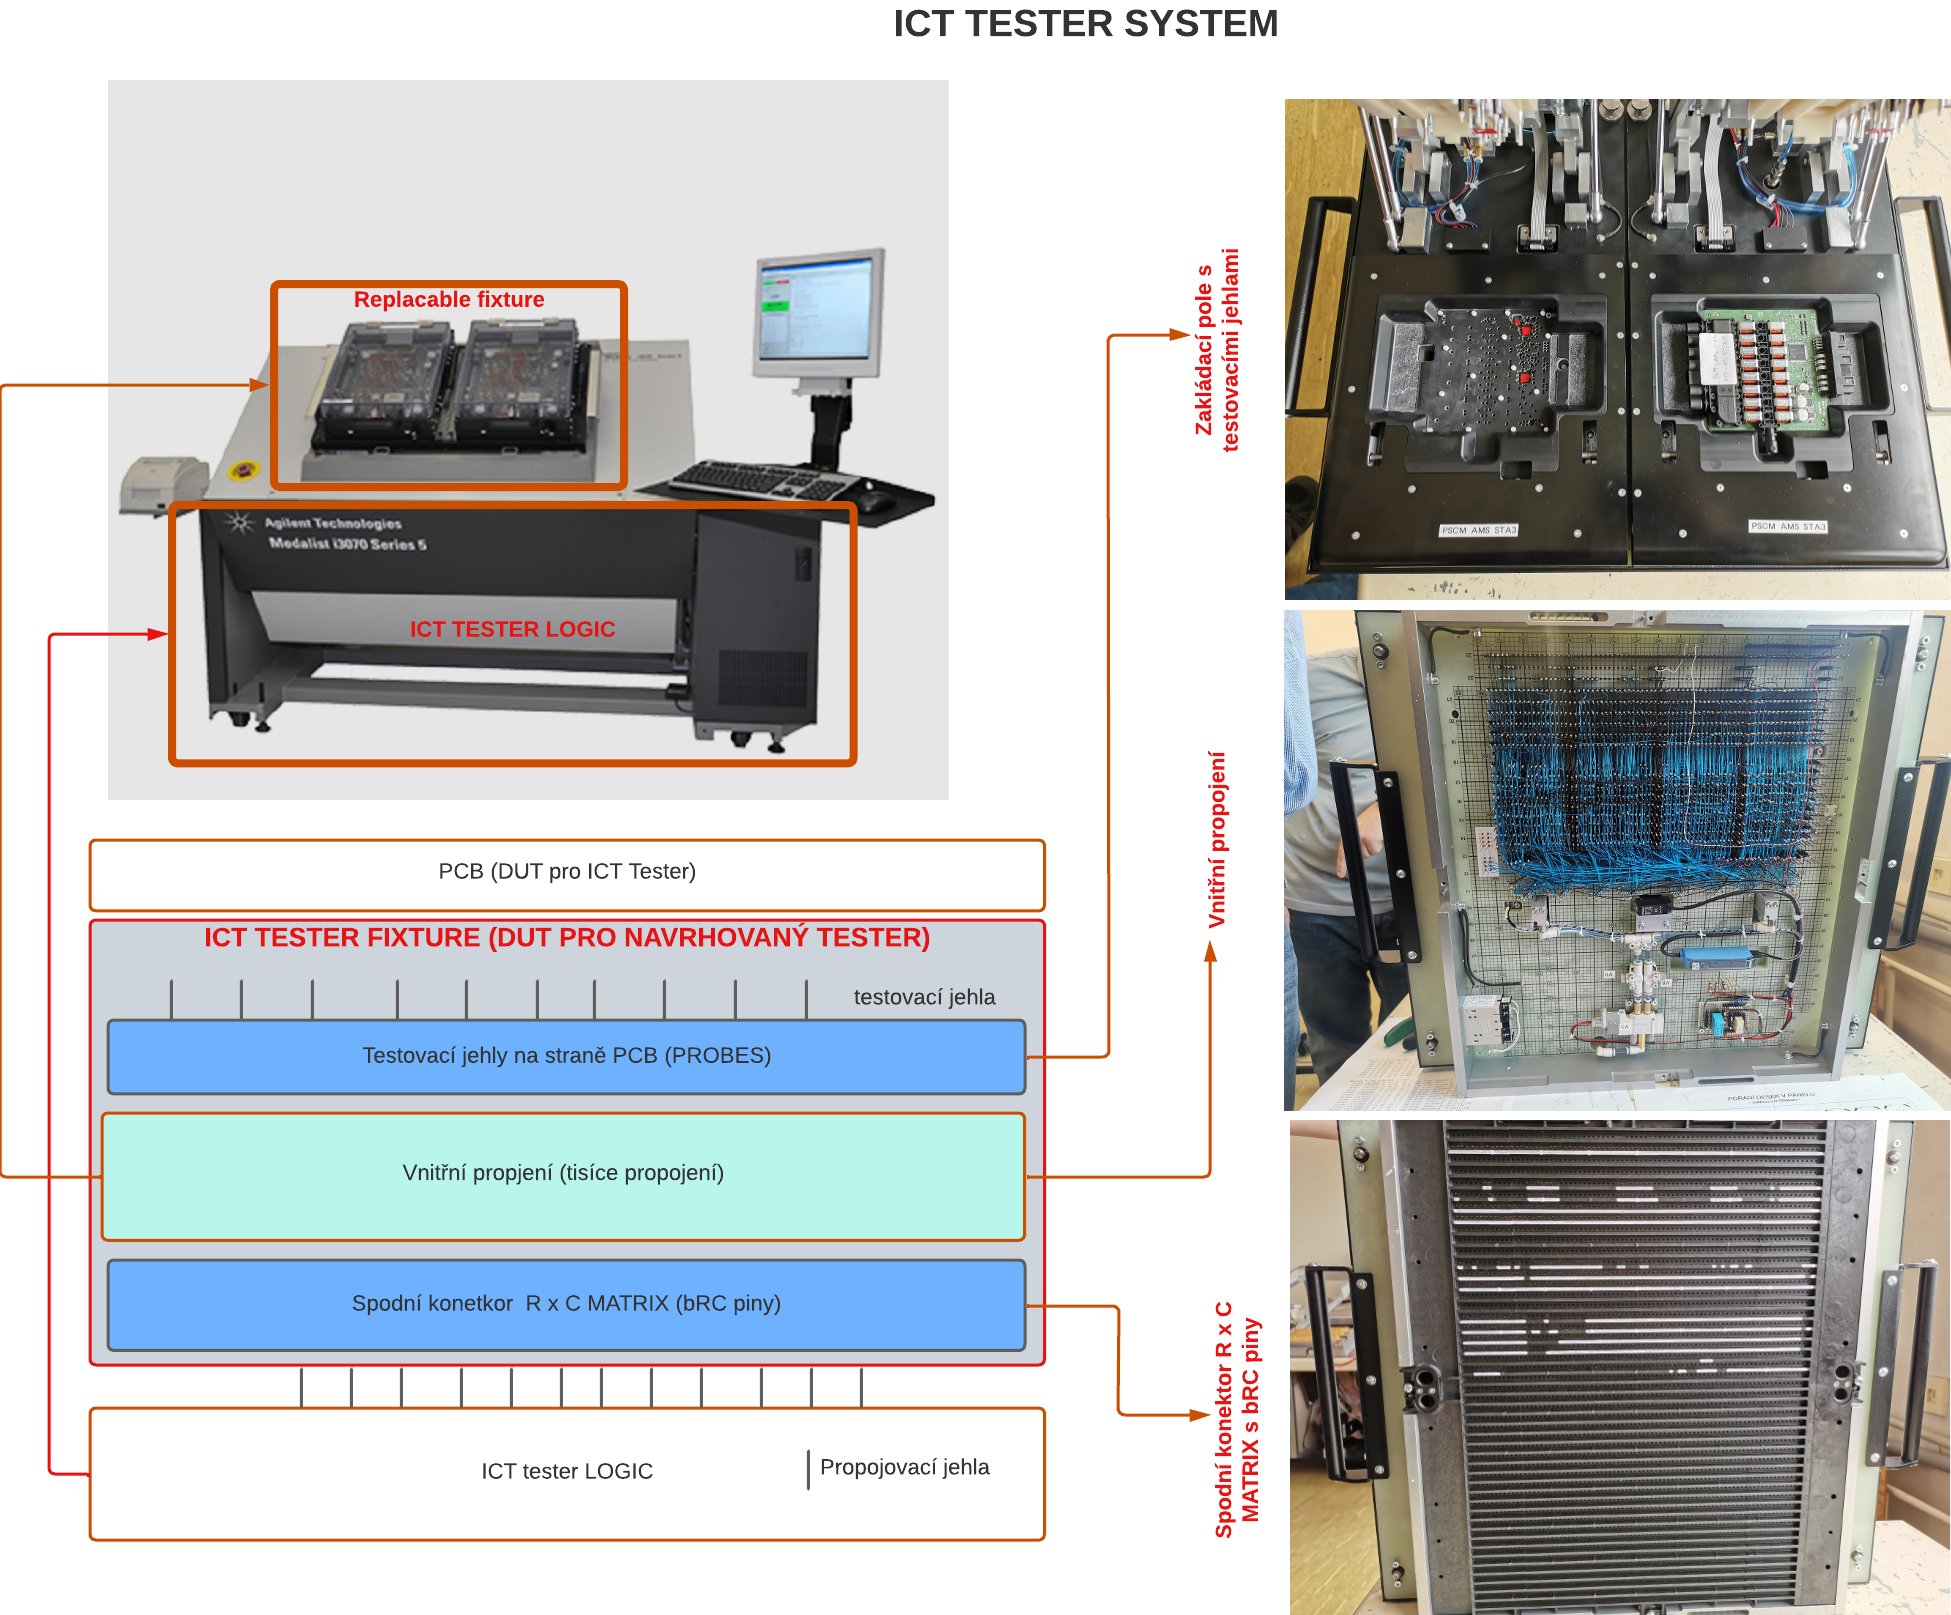
\includegraphics[width=0.9\textwidth]{obrazky/ICT_tester.png}
    \caption{Části ICT testeru (obrázek testeru vlevo nahoře převzat z \cite{ICT_picture})}
    \label{fig:ICT_tester}
    \end{figure}
    \clearpage

\section{Koncepce navrhovaného testeru}
    Zatímco pro ICT tester bylo úkolem otestovat vložené PCB. Úkolem zařízení,
    navrhovaným v diplomové práci, je otestovat správnost propojení
    fixture části ICT testeru. Pro tento účel je navržena následující koncepce.

    \begin{figure}[ht!]
        \centering
        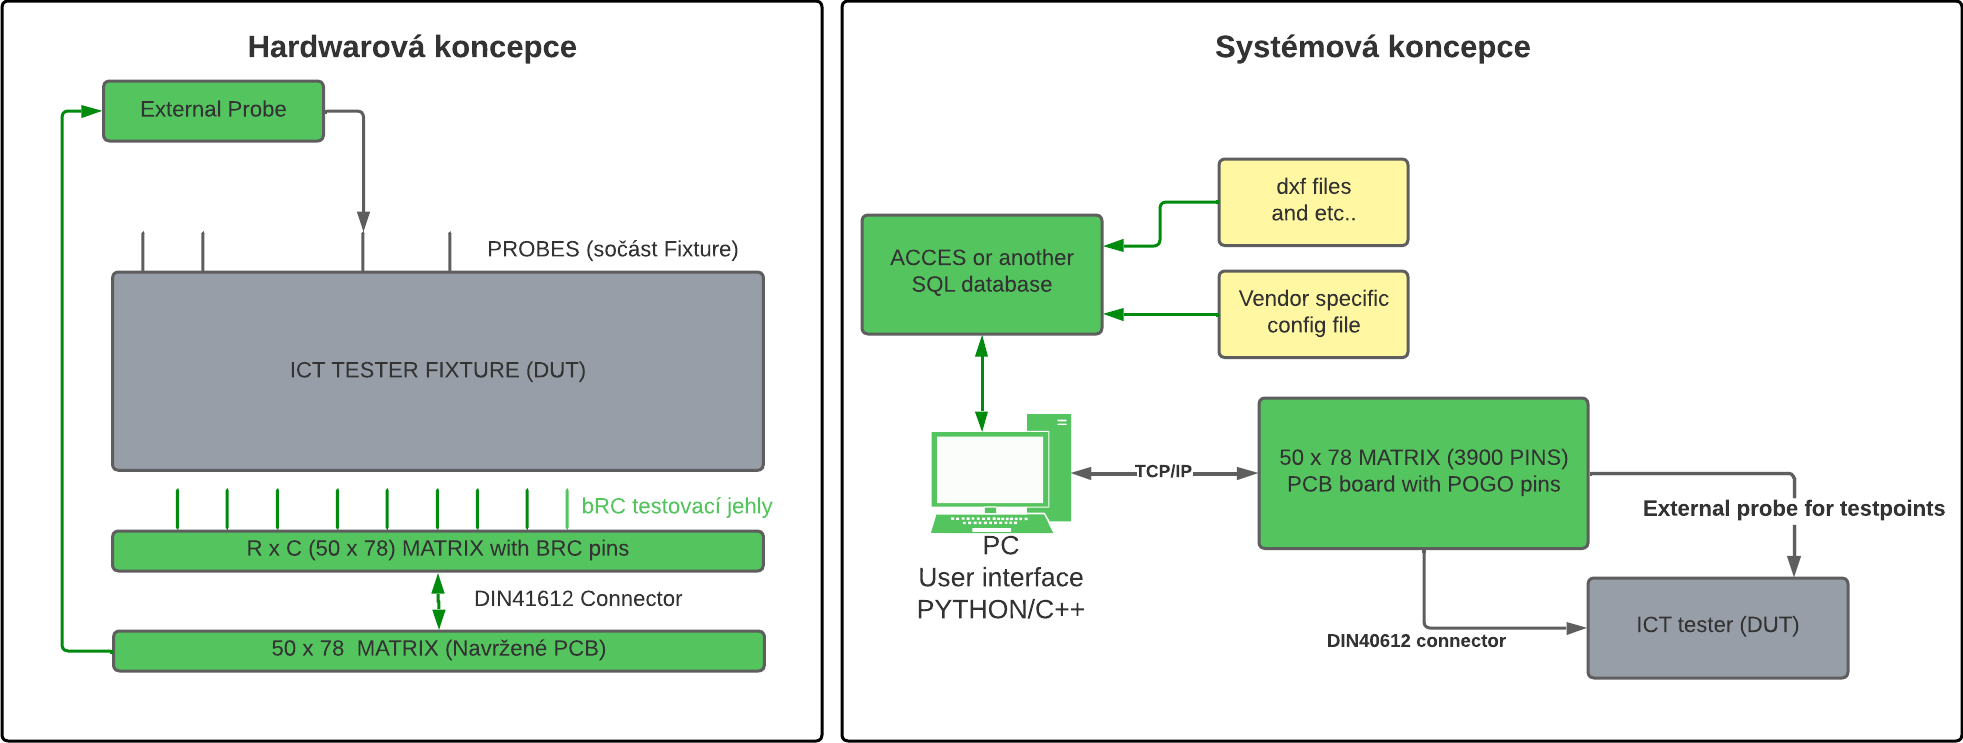
\includegraphics[width = 1\textwidth]{obrazky/system_connection_and_fixture.png}
        \caption{Koncepce funkčnosti navrhovaného testeru}
        \label{fig:Koncepce funkce}
    \end{figure}

    Na obrázku \ref{fig:Koncepce funkce} jsou zeleně znázorněny části, která jsou součástí diplomové práce.
    Ostatní barvy značí části, které již existují a nebudou navrhovány.

    \subsection{Systémová koncepce}
    Na obrázku \ref{fig:Koncepce funkce} v pravé části je znázorněná systémová koncepce testeru.
    Pro otestování vnitřního propojení fixture je nutné propojit všechny bRC piny s logikou navrhovaného testeru.
    Většina komerčních ICT testerů omezuje počet sloupců v bRC MATRIX na 78 a liší se tak pouze počtem řad.
    Z tohoto důvodu je tester navržen tak, aby bylo možné libovolně  měnit počet řad o 78 pinech\cite{ICT_guidline}.
    
    \begin{figure}[ht!]
        \centering
        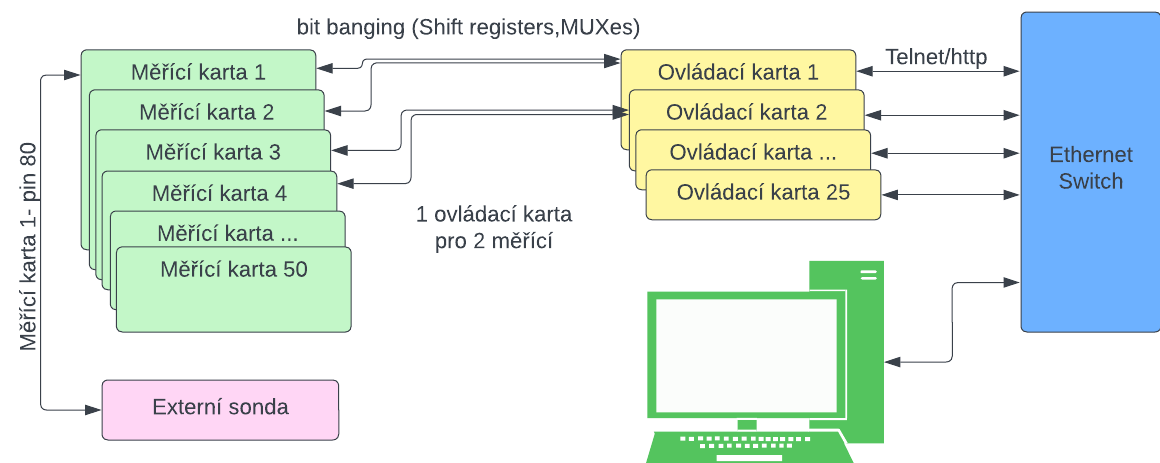
\includegraphics[width = 1\textwidth]{obrazky/telnet_http_pc.png}
        \caption{Systémová koncepce}
        \label{fig:Systémová koncepce}
    \end{figure}\par
    \clearpage
    Navržené zařízení se skládá z měřících karet,
    ovládacích karet a řídícího počítače \mbox{(Obr. \ref{fig:Systémová koncepce})}.
    Úkolem měřící karty je měřit hodnoty odporu mezi jednotlivými bRC piny
    a odesílat data do ovládací karty. Měřící karty jsou kompatibilní s 5V a 3V3 logikou.
    \begin{figure}[ht!] 
        \centering
        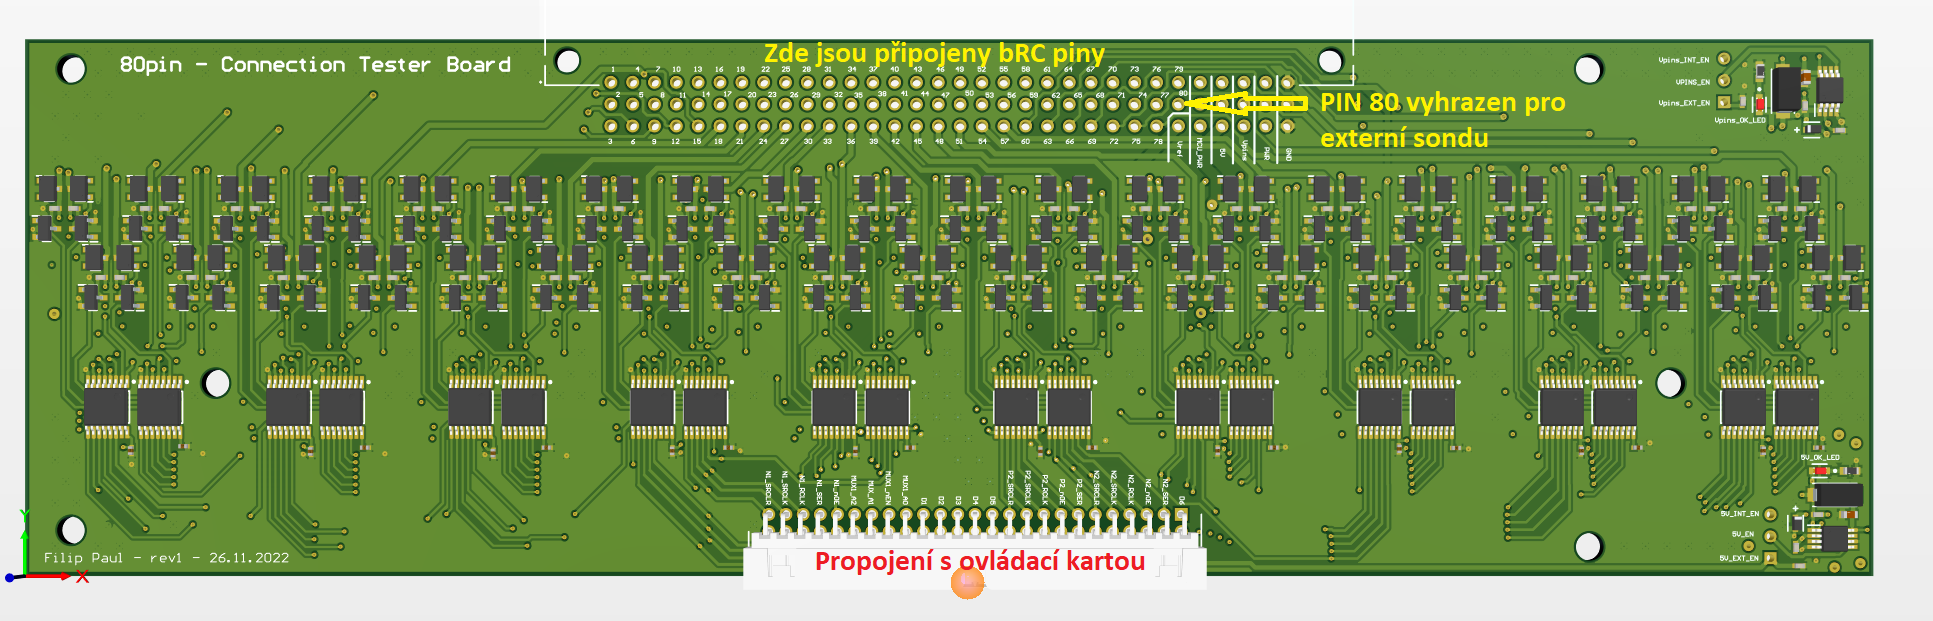
\includegraphics[width = 0.95\textwidth]{obrazky/karta_3D_NP.png}
        \caption{Měřící karta}
        \label{fig:Měřící karta}
    \end{figure}

    \begin{figure}[ht!]
        \centering
        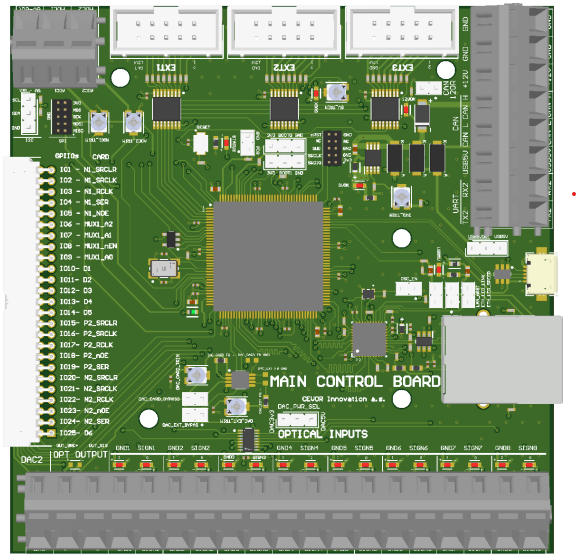
\includegraphics[width = 0.7\textwidth]{obrazky/3D_ovl_karta.png}
        \caption{Ovládací karta - 3D model}
        \label{fig:Ovládací karta - 3D model}
    \end{figure}
    Jednotlivé ovládací karty mají možnost připojení k ethernetové síti pomocí
    \mbox{100BASE-T} a jsou schopny ovládat měřící karty.
    Ovládací karty komunikují pouze s řídící PC aplikací (nikoliv mezi sebou).
    Řídící PC aplikace řídí všechny testy. Ovládací karty mají v sobě implementován Telnet a http server,
    přičemž se pro hlavní komunikaci používá právě Telnet server.
    Takto lze využít jakékoliv zařízení s přístupem do sítě pro řízení testeru.\par
    
    Řídící aplikace využívá ke své činnosti celou řadu vstupních souborů. Jedná se o soubory, které definují zapojení fixture, CAD, CAM a další data\cite{CAD_wiki}.
    Protože vstupní soubory nemají jednotný formát pro každého výrobce, aplikace nejprve data převede do mySQL databáze. S takto zpracovanými daty již lze
    provádět jednotné operace. Aplikace porovnává naměřená data z jednotlivých karet ze vstupními soubory a následně generuje výsledek testu propojení
    v co nejsrozumitelnější podobě.

    \subsection{Hardwarová koncepce}
    \subsubsection{Propojení bRC pinů mezi sebou}
    Propojení mezi měřícími kartami a maticí bRC pinů je zajištěno pomocí POGO pinů (strana fixture),
    bRC jehel (strana testeru) a pneumatického kontaktování.
    Na Obr. \ref{fig:Měřící karta} je znázorněn 3D model měřící karty. V horní části jsou připraveny 
    body pro připojení bRC jehel a napájení desky. Rozteč kontaktů je zvolena tak, aby bylo možno
    k měřící kartě připájet standardizovaný DIN41612 konektor (dále pouze DIN) a kartu tak snadno použít pro jiné aplikace.\par

    Ve spodní části se nachází 25x2 konektor, sloužící k propojení s ovládací kartou. Měřící karta je navržena tak, aby buď poskytovala
    napájení ovládací kartě anebo byla ovládací kartou napájena (více v sekci o návrhu měřící karty).

    \subsubsection{Propojení mezi bRC a Probes}
    Pomocí karet je možné automaticky zjistit propojení mezi všemi bRC piny,
    nicméně přímé propojení mezi bRC a Probe piny je nutné otestovat zvlášť.
    Za tímto účelem je k testeru připojena externí sonda (Obr. \ref{fig:Systémová koncepce}).
    Sonda je připojena do bRC pinu \hbox{č. 80} na měřící
    kartě \hbox{č. 1.}\\

    Obsluha v závislosti na pokynech PC aplikace připojuje sondu k jednotlivým probes pinům.
    Takto lze pomocí jednotlivých karet zjistit propojení.
    Externí sonda je podobná jako sonda multimetru a slouží pouze k přivedení testovacího napětí na probe pin.
    Proces lze celý automatizovat v případě, že je k dispozici i maketa PCB,
    která bude obsahovat všechny probe piny přivedené na DIN konektor.
    V takovém případě lze připojit maketu PCB ke kartě a proces automatizovat.